%% Default Latex document template
%%
%%  blake@rcs.ee.washington.edu

\documentclass[letterpaper]{article}

% Uncomment for bibliog.
\bibliographystyle{unsrt}

\usepackage{graphicx}
\usepackage{lineno}
\usepackage{amsmath}

%\usepackage{fancyhdr}

%%%%%%%%%%%%%%%%%%%%%%%%%%%%%%%%%%%%%%%%5
%
%  Set Up Margins

%%%%%%%%%%%%%%%%%%%%%%%%%%%%%%%%%%%%%%%%%%%%%%%%%
% include file for:
%      Critical Page setup dimensions
%            DO NOT MODIFY
%       (for help see "Latex Line by Line" p 260)
%
\setlength\oddsidemargin{0in}
\setlength\evensidemargin{0in}

\usepackage[left=0.98in, right=0.98in, top=1.0in, bottom=1.0in]{geometry}

% %Top Margin and header
% \setlength\voffset{-0.94in}
% \setlength\topmargin{0.25in}
% \setlength\headheight{0.25in}
% %\setlength\headwidth{6.5in}
% \setlength\headsep{0.25in}
% %Body
% \setlength\textwidth{6.5in}
% \setlength\textheight{9.50in}
% %Footer
% %\setlength\footheight{0.5in}
% \setlength\footskip{0.3750in}
% Line spacing for 6 lines per inch
\linespread{0.894}  % 1.0 = single    1.6 = double
%
%          END of Critical Page Setup Dimensions
%%%%%%%%%%%%%%%%%%%%%%%%%%%%%%%%%%%%%%%%%%%%%%%%%%%

%%%%%%%%%%%%%%%%%%%%%%%%%%%%%%%%%%%%%%%%%%%%%%%%%%%
%
% Useful style and math macros
%


\newcommand\Dfrac[2]{\frac{\displaystyle #1}{\displaystyle #2}}
\newcommand\beq{\begin{equation}}
\newcommand\eeq{\end{equation}}

\newcommand\bmat{\begin{bmatrix}}
\newcommand\emat{\end{bmatrix}}

\newenvironment{solution}
{\ttfamily \vspace{0.155in} {\bf SOLUTION:} \\ }
{ \vspace{0.25in} \par }



%
%        Font selection
%
%\renewcommand{\rmdefault}{ptm}             % Times
%\renewcommand{\rmdefault}{phv}             % Helvetica
%\renewcommand{\rmdefault}{pcr}             % Courier
%\renewcommand{\rmdefault}{pbk}             % Bookman
%\renewcommand{\rmdefault}{pag}             % Avant Garde
%\renewcommand{\rmdefault}{ppl}             % Palatino
%\renewcommand{\rmdefault}{pch}             % Charter


%%%%%%%%%%%%%%%%%%%%%%%%%%%%%%%%%%%%%%%%%%%%%%%%%
%
%         Page format Mods HERE
%
%Mod's to page size for this document
\addtolength\textwidth{0cm}
\addtolength\oddsidemargin{0cm}
\addtolength\headsep{0cm}
\addtolength\textheight{0cm}
%\linespread{0.894}   % 0.894 = 6 lines per inch, 1 = "single",  1.6 = "double"

% header options for fancyhdr

%\pagestyle{fancy}
%\lhead{LEFT HEADER}
%\chead{CENTER HEADER}
%\rhead{RIGHT HEADER}
%\lfoot{Hannaford, U. of Washington}
%\rfoot{\today}
%\cfoot{\thepage}



% Make table rows deeper
%\renewcommand\arraystretch{2.0}% Vertical Row size, 1.0 is for standard spacing)

\begin{document}
\begin{centering}
{\Large   Simulation of Everting Tube Experiments}

Blake Hannaford

\today

\end{centering}

\section{Introduction}

\subsection{Literature Review}

Prior studies of eversion mechanics have relied on the assumption of constant
pressure over time and throughout the extent of the device.
\cite{blumenschein2017modeling}
Applied biomechanical models for plant shoot growth to analogous physical
processes in everting tubes and combined it with experimental measurements.
Notably, for their speeds and design parameters, they did not find an
effect of air flow drag caused by filling the everting tube.
\cite{Hawkes2017} Performed mostly quasi-static modeling of ETs
but studied the important buckling phenomena in complex geometric
environments.
\cite{vartholomeos2024lumped} created a dynamic, lumped parameter
mechanical model
of eversion with special emphasis on friction properties between
an everting tube and its environment as well as a second contact
between the tube and a rod (catheter) in contact with the
everted material.

\subsection{Observed Eversion Characteristics}

\begin{figure}[h]\centering
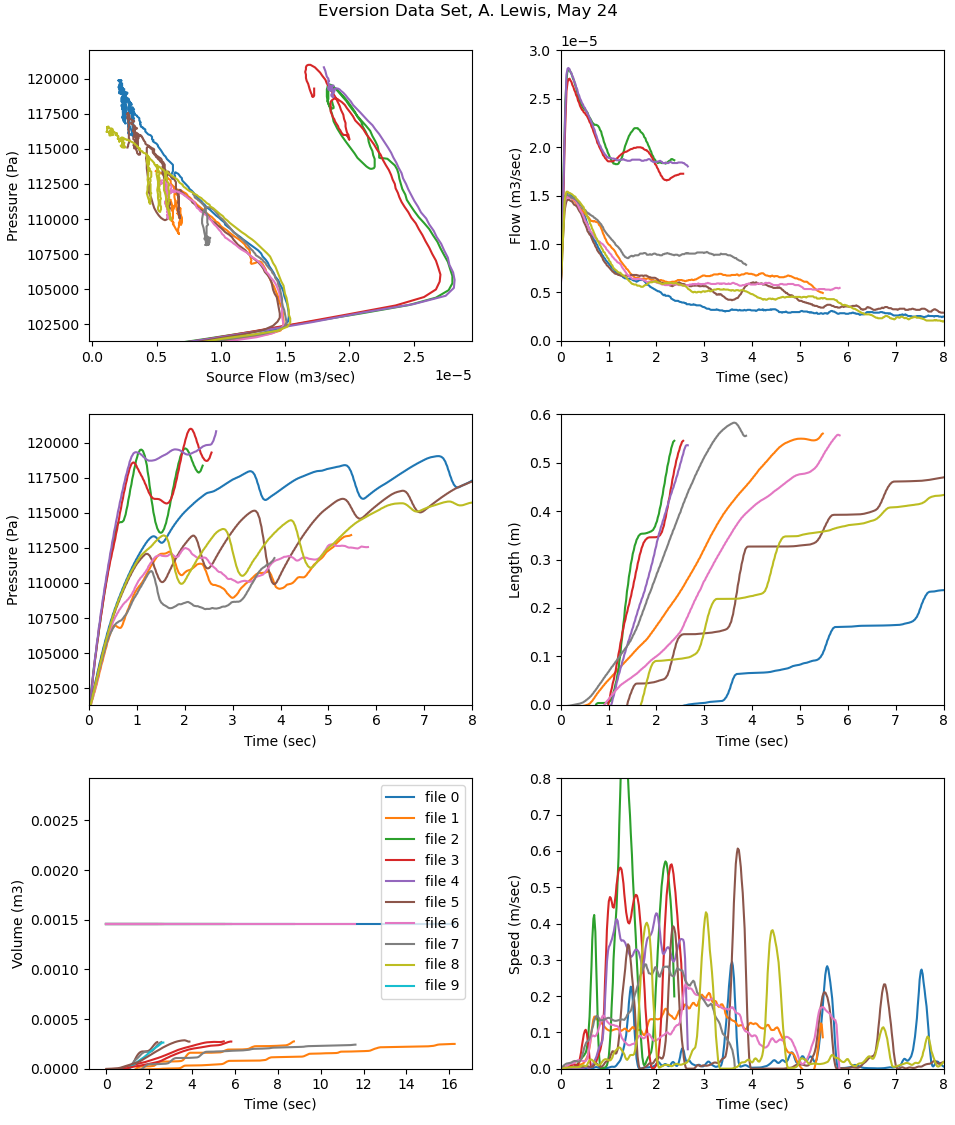
\includegraphics[width=.475\textwidth]{ExpDataExampleAll.png}
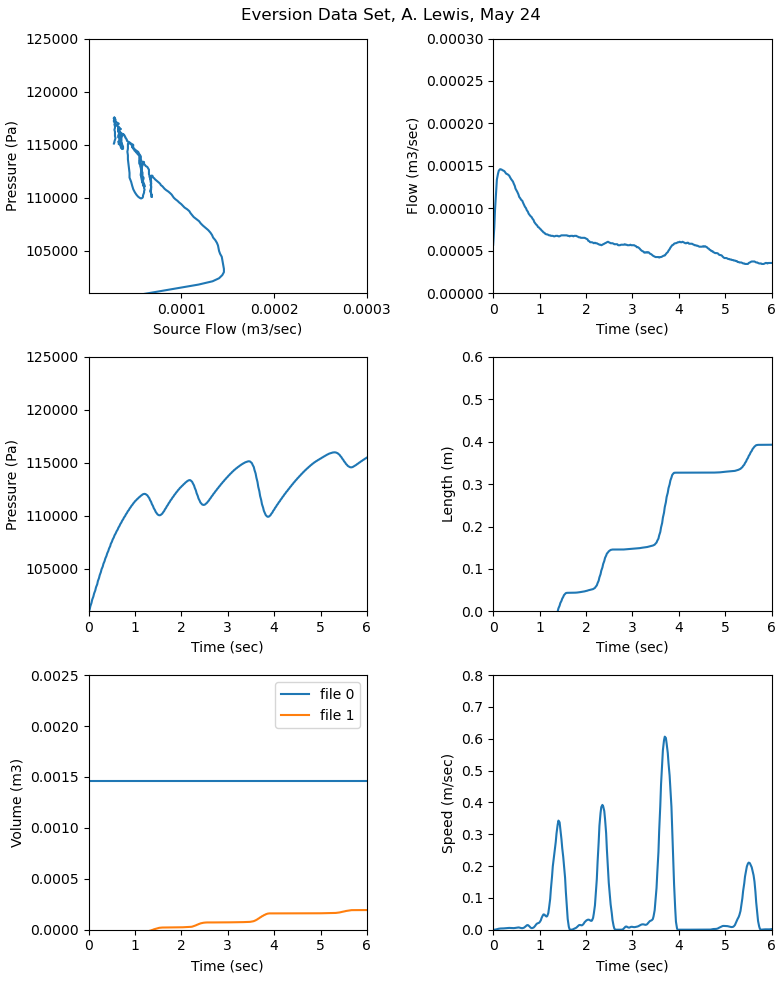
\includegraphics[width=.475\textwidth]{ExpDataExample.png}
\caption{Experimental data displaying dynamic characteristics of loaded eversion.  All data (Left), single example (Right) (See Lewis, Fig 9. Loads: high inertia, high Friction)}
\label{Fig:experData}
\end{figure}

Some theory of everting tubes has been reviewed above.   Complex dynamic behaviors of a tube everting
inside
a straight tube of approximately the same diameter as the inflated tubing material were measured
by Lewis \cite{xxxx} (Figure \ref{Fig:experData}, Left panel).
There seem to be two distinct clusters of responses, five slower and three faster (particularly clear
in the flow plots (top row).
One experiment which displays several interesting everting characteristics
is shown in Figure \ref{Fig:experData}, Right Panel.
Referring first to the length-vs-time plot (middle right), we see a start-stop or staircase
behavior sometimes seen with eversion under relatively constant input pressure.   It
should be noted that the selected eversion experiment (Right panel) was loaded by reel inertia and
by friction applied to the reel.  Velocity (lower right) indicates a series of peaks where the eversion
``breaks-free" but then stops again a short time later giving length-vs-time a stair-step characteristic.

Pressure (middle left) first grows for about 1 second without corresponding eversion motion, and
then oscillates in approximate synchrony with the velocity peaks.

Finally, the pressure-flow phase plot (top left) shows diagonal slope (the trajectory proceeds from
lower right (high initial flow with low pressure) to upper left (lower flow, higher pressure).
The trajectory makes loops to lower pressures and back up to the slope at higher pressures.  These
loops correspond in time to the pressure oscillations (middle left).

These dynamic characteristics (start-stop bursting, pressure oscillations, diagonal phase trajectory, and
downward loops) were not all present under all experimental conditions.  In summary then, depending on
factors to be determined, some or all of these characteristics may or may not be present in a given
eversion run.

\subsection{Simulation Goals}
The goals of this simulation are:
\begin{enumerate}
  \item Increase fundamental understanding of the eversion process.
  \item Identify key parameters capable of representing the complex dynamic characteristics above.
  \item Identify values and value ranges for unknown parameters which fit individual experiments.
  \item Clearly segregate the parameters into known, measured quantities vs. free parameters.
  \item Codify an efficient manual method for parameter identification.
\end{enumerate}

In any simulation study caution must be exercised when there are a large number of free parameters
as there may be several combinations of parameters or manifolds in the parameter space which
may fit any dataset.   In Section \ref{xxxxx}, below, we review the overall parameter set and
classify the parameters into known, independently measureable parameters vs free parameters.


\subsection{Dynamic Model}
The dynamic model of an eversion drive system includes;
\begin{itemize}
  \item An everting tube of length $L$ and growth rate $\dot{L}$.
  \item A pressurized housing
  \item A reel with rotation $\theta, \dot{\theta}, \ddot{\theta}$, on which tubing is rolled having inertia (assume fixed) of
  $J$ and radius $r$.
  \item A brake which applies a Coulomb friction torque to the reel
  \[
    \tau_c = C\mathrm{sgn}(\dot{\theta})
  \]
  \item A ``crumple zone" in which eversion material can accumulate
  between the reel and the everting tube. The length of material in
  the crumple zone is $L_c$.
  \item Eversion happens when the eversion force (pressure $\times$ face area of the tube) exceeds any retarding forces.
  \item Forces which can oppose eversion include,
  \begin{itemize}
    \item drag forces inertial forces required to pull the tubing material
    inside the deployed tube,
    \item reel inertia and reel friction resulting from unspooling material,
  \end{itemize}
\end{itemize}

\noindent
The everting tube can be in one of two states:
\begin{itemize}
  \item GROWING (the tube is actively everting, $\dot{L}>0$)
  \item STUCK (the tube is not growing due to insufficient everting force, $\dot{L}=0$)
\end{itemize}
and the reel/crumple zone can be in one of two additional states:

\begin{itemize}
  \item TAUGHT (the crumple zone has zero length , $L_c = 0 $)
  \item SLACK (there is material in the crumple zone, $L_c > 0$)
\end{itemize}

Together the system can be in four states comprising the permutations
of these two state variables.

\section{System Equations:}

After setting initial conditions (see below), we model eversion dynamics by:
\begin{enumerate}
  \item Computing pressure, volume, and flow from the source.
  \item Computing forces applied to the eversion tip.
  \item Accounting for the mechanical advantage (everting material speed is $2\times\dot{L}$, Pressure applied to everting front develops 1/2 the everting force expected from $P\times A$.)

  \item Selecting the dynamic mode from the four combined states above.
  GROWING and STUCK are selected by force thresholds applied to net
  eversion force.    TAUGHT and SLACK are selected by checking length of
  the crumple zone material.

  \item According to the dynamic mode, summing forces, equating to  zero, solving for tube and reel accelerations.
  \item Eversion does not come to an instant halt. We  empirically model exponential decay of velocity as tube decelerates.
\end{enumerate}

\noindent
Specifically:

\begin{equation}\label{eqOneCompartmentVol}
V_t = V_{housing} - V_{contents} + L  A
\end{equation}
$V_t$ includes both the reel housing minus the volume of its contents,
and the everted tube of length $L$ with cross sectional area $A$.

From the ideal gas equation:
\begin{equation}\label{eqOneCompartmentPress}
P = \frac{N  RT}{ V_t}
\end{equation}
where $N$ is the molar mass of gas in the system, $R$ is the gas constant, and $T$ is the temperature
in $^\circ$K, (which we assume is constant).

\begin{figure}\centering
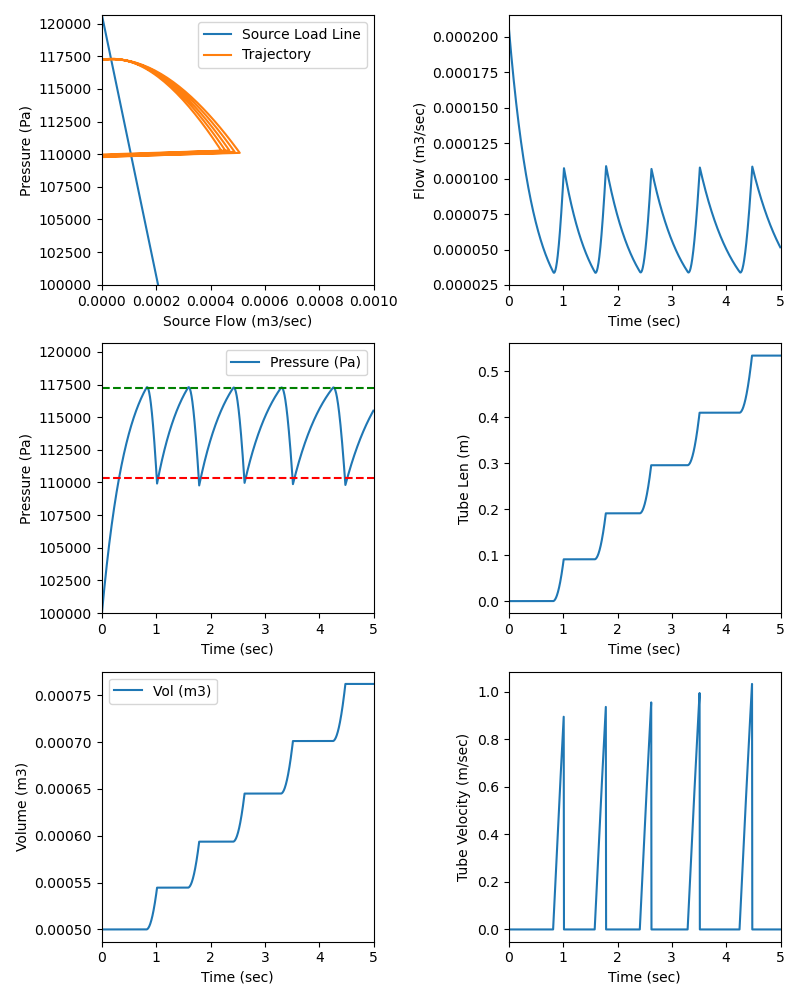
\includegraphics[width=.75\textwidth]{Figure_9HhiI_hiTf_baseline.png}
\caption{Simulation Run with approximate qualitative match.  (See Lewis, Fig 9, hiI, hiTf)}
\label{Fig:baselineResults}
\end{figure}

Computing Forces:


\begin{equation}
  F_{ever} = \mathrm{max}(0, PA/2)
\end{equation}
\beq
  F_{c} = \tau_{Coulomb} / r
\eeq

Coulomb friction is independent of velocity so does not get scaled by the $2\times$ mechanical advantage.

Computing acceleration according to the dynamic state:

GROWING and SLACK:

\beq
\ddot{L} = \frac{F_{ever} - F_D(L,\dot{L})-F_C}  {M_T}
\eeq
\beq
\dot{\theta} = \tau_{Coulomb}/J
\eeq

GROWING and TAUGHT:

%         Lddot = (1/Mt + (rReel\_SIu**2/J) ) * ( F_ever - Fdrag(L,Ldot) - Fcoulomb )
%         th_ddot = Lddot/rReel\_SIu
\beq
\ddot{L} =(F_{ever} - F_D - F_C) /  (M_T + J/r^2)
\eeq

\beq
\ddot{\theta} = \ddot{L}/r
\eeq

STUCK and (SLACK or TAUGHT):


%         alpha = 2000 * dt  # empirical fit
%         Lddot = -1 * max(0, alpha * Ldot)
%         th_ddot = tau_coulomb/J

\beq
\ddot{L} = -1 * \mathrm(max)(0, \alpha * \dot{L})
\eeq

\beq
\ddot{\theta} = \tau_{Coulomb} / J
\eeq
where $\alpha$ is an empirical time constant modeling the dynamics of eversion stopping.

Modeling flow from the pressure source (Thevenin equivalent):
\begin{equation}\label{eqOneCompartmentflow}
Fl_{source} = \frac {P_{source}-P} {R_{source}}
\end{equation}

Converting airflow ($m^3/sec$) to rate of molar mass flow:
\begin{equation}\label{eqOneCompartmentNdot}
\dot{N} = Fl_{source} \cdot \mathrm{moles\_per\_m3}
\end{equation}

Model velocity and length dependent eversion force which is resistance to pulling out eversion material:
\begin{equation}
F_D(L,\dot{L} = 2 L  K_D  \dot{L}
\end{equation}

Where the factor of two accounts for everting material going at twice tube growth rate, $\dot{L}$.

Update length of  crumpled material (if any)
\beq
L_C = \mathrm{max}(0,  r\theta - L)
\eeq

We have a switching model to replicate observed intermittent starting and stopping of eversion
which updates the state based on current pressure:
\begin{equation}
    \mathtt{state} =
    \begin{cases}
      \mathrm{GROWING}, &  P > P2 \\
      \mathrm{unchanged}, & P1 <= P <= P2 \\
      \mathrm{STUCK},   &  P < P1
    \end{cases}
\end{equation}



We are currently investigating changing this switching model to one based on thresholding
net eversion force rather than tip surface pressure:
\begin{equation}
    \mathtt{state1} =
    \begin{cases}
      \mathrm{GROWING},   &  F_{ever} > F2 \\
      \mathrm{unchanged}, &  F1 <= F_{ever} <= F2 \\
      \mathrm{STUCK},     &  F_{ever} < F1
    \end{cases}
\end{equation}

In either case above, we update the crumple state as
\begin{equation}
    \mathtt{state2} =
    \begin{cases}
      \mathrm{TAUGHT},  &  L_C <=0 \\
      \mathrm{SLACK},   &  L_C  > 0
    \end{cases}
\end{equation}

Finally, we integrate the state variables:
\begin{equation}
\begin{aligned}
  \dot{L} &= \dot{L} +  \ddot{L}  dt \\
  L       &= L + \dot{L}  dt \\
  \dot{\theta} &= \dot{\theta} + \ddot{\theta}dt \\
  \theta &= \theta + \dot{\theta} dt\\
  N &= N + \dot{N}  dt\\
\end{aligned}
\end{equation}


\subsection{Initial Conditions}
\begin{equation}
\begin{aligned}
  P &= 1 \; \mathrm{atmosphere}\\
  {\tt state1} &= STUCK \\
  {\tt state2} &= TAUGHT \\
  N &= N(V_{housing} - V_{contents}) / RT \\
  L &= 0\\
  \dot{L} &= 0\\
  \ddot{L} &= 0\\
\end{aligned}
\end{equation}

\subsection{Parameters}
The model parameters are classified in Table \ref{Tab:paramClass}

\begin{table}
\begin{tabular}{l|l|l|l|l|l}
Parameter     &  Class     & Value   & Units     & Description      & source \\ \hline
ET\_radius     &  Known     & 12.5    &  $mm$       & Tube radius      & tube design \\
J             &  Known     & 5.1E-4 &  $kg/m^2$    & Reel inertia     & design and testing \cite{Lewis2024XX} \\
Lmax          &  Known     & 0.5-0.8 &  $m$        & Tube length      & tube design \& fitting \\
Patmosphere   &  Known     & 101.325 &  $kPa$      & Atmospheric pressure & \\
RT            &  Known     & 2.5E+3 &   $m^3 Pa/mol$   & Gas constant x temperature &  \\
T             &  Known     & 2.95E+2 &  $^\circ K$    & Room temperature   & Thermometer \\
Tau\_coulomb   &  Known     &        &  $Nm$       & Coulomb fric. torque on reel  & design and testing \cite{Lewis2024XX} \\
Vhousing\_m3   &  Known     &  1.5E-3&  $m^3$      & Net housing air volume  & CAD model \\
et\_MPM        &  Known     &  0.1    &  $kg$       & Tubing mass per meter  & measured \\
rReel         &  Known     &         &   $m$       & Reel radius & CAD model \\ \hline
K2drag        &  Free      &         &  $Nm$       & Empirical Fit    & manual tuning \\
Kdrag         &  Free      &         &  $N/m^2/sec$ & Empirical Fit & manual tuning \\
PBA\_static    &  Free      &         &  $kPa$      & Break-away pressure  & manual tuning \\
PHalt\_dyn     &  Free      &         &  $kPa$      & Eversion stopping press.  & manual tuning \\
Psource\_SIu   &  Free      & 0-20    &  $kPa$      & Gas source pressure & manual tuning\\
Rsource\_SIu   &  Free      & 1.0E8   &  $Pa/m^3$    & Slope of P-Fl load-line & manual tuning\\
Threshold Taper & Free     &          &  $Pa/m$      & Change in PBA w/ length   & manual tuning\\
% Observation         & Param       & Orig. value   &  Modified Value  \\\hline
% Velocities too high  & ${\tt Kdrag}$  &   0.3     & 0.6          \\\hline
% Pressure thresholds converge with time& {\tt PBA\_static} & $1.17\times10^5 $Pa & $1.17\times10^5 - 500L$ Pa          \\\hline
% Pressure thresholds converge with time & {\tt PHalt\_dyn} & $1.17\times10^5 $Pa & $1.013\times10^5 + 500L$ Pa       \\\hline
% Pressure rise too slow  & $V_{housing}$   &  $0.5\times10^{-3}$ m$^3$   & $0.05\times10^{-3} $ m$^3$   \\\hline
% Peak Velocity too high  & $J$             &  $5.10\times10^4$  kg/m$^2$     & 10.2$\times10^4$  kg/m$^2$ \\\hline
\end{tabular}
\caption{Parameters used and their sources and values. }
\end{table}\label{Tab:paramClass}

\vspace{0.175in}

The modified parameter set is given in Section \ref{modParams} below.  Asterisks (*) denote iteratively changed parameters.

Simulation with the modified parameters (Figure \ref{Fig:ModifParResults}) improve the model fit to data by
    1) Shrinking loops on the pressure flow plot (upper left) are similar
  to shrinking loops in experimental pressure-velocity plot'
    2) Convergence of the eversion thresholds (center left) causes the shrinking loops above,
    3) Peak velocities better match peaks of fig. 9, and match the pattern of the highest velocity
  appearing near the center of travel.
    4) With the modified parmeters there are about 2 bursts per second, similar to the experimental rate.



\begin{figure}\centering
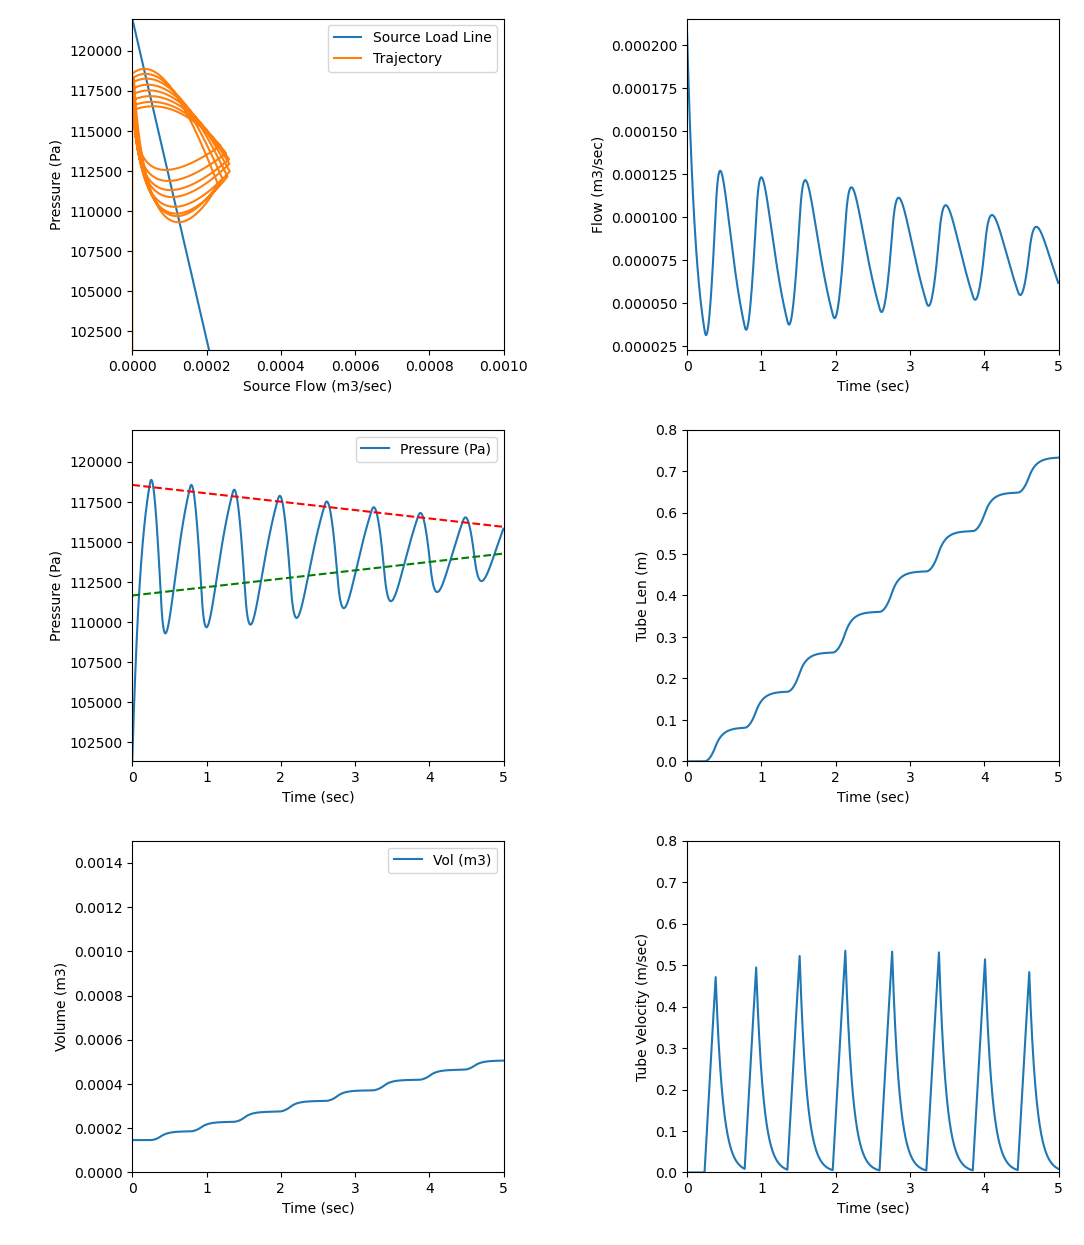
\includegraphics[width=.75\textwidth]{Figure_9HhiI_hiTf_tweakedParams.png}
\caption{Improved qualitative match with modified parameters.  (See Lewis, Fig 9, hiI, hiTf)}
\label{Fig:ModifParResults}
\end{figure}

\clearpage

\section{Baseline Parameter Values}\label{baselineParms}
\begin{verbatim}

      moles_per_m3   4.4623E+01  moles / m3
      Psource\_SIu    1.2066E+05  Pascals
      LLine\_SIu      1.0000E-08  m3/sec / Pascal
      Rsource\_SIu    1.0000E+08  Pa/m3/sec
      Vhousing_m3    1.4616E-03  m3
      Kdrag          3.0000E-01  N / m2 / sec
      area_m2        4.9087E-04  m2
      Pintercept     1.2066E+05  Pascals
      Fintercept     2.0684E-04  m3/sec
      Vintercept     4.2137E-01  m/sec
      PBA_static     1.1721E+05  Pascals
      PHalt_dyn      1.1032E+05  Pascals
      Patmosphere    1.0132E+05  Pascals

\end{verbatim}


\section{Modified Parameter Values}\label{modParams}
\begin{verbatim}

      moles_per_m3   4.4623E+01  moles / m3 of Air
      Patmosphere    1.0132E+05  Pascals
      Psource\_SIu    1.2201E+05  Pascals
      LLine\_SIu      1.0000E-08  m3/sec / Pascal
      Rsource\_SIu    1.0000E+08  Pa/m3/sec
      J            * 1.0200E-03  kg/m2
      Vhousing_m3  * 1.4616E-04  m3
      Kdrag        * 1.2000E+00  N / m2 / sec
      area_m2        4.9087E-04  m2
      Pintercept     1.2201E+05  Pascals
      Fintercept     2.0684E-04  m3/sec
      Vintercept     4.2138E-01  m/sec
      Threshold Taper *   3.5714E+03  Pa /m
      PBA_static     1.1856E+05  Pascals
      PHalt_dyn      1.1167E+05  Pascals

\end{verbatim}

\section{Parameter Estimation from Data}

The following process can be used to fit parameters to an eversion data record where the record consists of
the following data as a function of time:

\begin{itemize}
    \item Pressure in the tube storage chamber (Pa)
    \item Air flow from source into tube storage chamber ($m^3/sec$)
    \item Length of everting tube relative to chamber opening (m)
    \item Velocity of eversion (derived) ($m/sec$)
\end{itemize}

These can be plotted multiple ways such as in Fig \ref{Fig:baselineResults} for example.

We can then use the following procedure to iteratively tune some of the  model  parameters to match a
particular experimental run.   Other parameters such as the tube reel radius, inertia, and braking
friction are readily measured independently \cite{Andy Papers}  and not fit to the eversion experiments.

\begin{enumerate}
    \item  Adjust load line pressure intercept.

    {\bf Data Focus: } Pressure/Flow curves (upper left):\\
    {\bf Procedure: } Adjust Psource\_SIu to move the load line and sim trajectory (they should overlap)
    up and down.  Adjust Rsource\_SIu to adjust its slope (higher values slope down more).

    \item Adjust stop-start thresholds.

     {\bf Data Focus: } Pressure-Time curves (middle left):\\
    {\bf Procedure: } Adjust PBA\_static up or down to match the pressure peaks in experiment (green dashed).
    Adjust PHalt\_dyn  up or down to match the pressure valleys.

    \item Adjust threshold taper.

     {\bf Data Focus: } Pressure-Time curves (middle left):\\
    {\bf Procedure: } Adjust Threshold Taper up or down to speed or slow down convergence of the thresholds.

    \item Adjust Friction or drag

     {\bf Data Focus: } Length-Time curves (middle right):\\
    {\bf Procedure: } Adjust the viscus drag constant of tubing (K\_drag) up or down to match the overall slope
    of the data trace.
    Adjust max tubing length (Lmax) to match stopping point of data.

    \item Experiment with other parameters or go back and repeat the procedure.

\end{enumerate}


\section{Model Refinements}

\subsection{Varying tube profile}

While most ET research uses tubing of constant diameter, the effective diameter of an ET can vary with
length in two main ways.   First, the tube can be fabricated with variable diameter by thermal welding of two sheets.
Second, tubing of constant diameter may be everted into a tubular space of changing diameters.
While the mechanics of eversion will in general be different in these two cases, we will initially ignore that difference
and make tube diameter a function of eversion distance $L$, $V(L)$.

Tube profiles

Simulations


\subsection{Multiple compartment model}
So far, pressure and flow dynamics have considered the tubing supply chamber and the everted tubing to be a single compartment
for computation of volume (Eqn \ref{eqOneCompartmentVol}) and pressure (Eqn \ref{eqOneCompartmentPress}) yielding a single
flow (Eqn \ref{eqOneCompartmentflow}).

In some experimental data [...details...]  we noted loops in the pressure-flow plane in which a growing ET deviated
significantly from the source load line.   This indicates that air pressure does not instantaneously equilibrate
along the ET, but instead takes time to flow from the tubing compartment down to new volume at the growing tip.
A lumped parameter model of this flow can be formed of two compartments, one is the reel housing from
which the tube is everted, and the second is
the tubing.   A flow resistance, $R_T(L)$, connects the two chambers and this resistance increases with length.
The tubing volume increases with length (as it did in Eqn \ref{eqOneCompartmentVol}).

Such a model is shown in Figure \ref{Fig:TwoCompartment}.


\begin{figure}[h]\centering
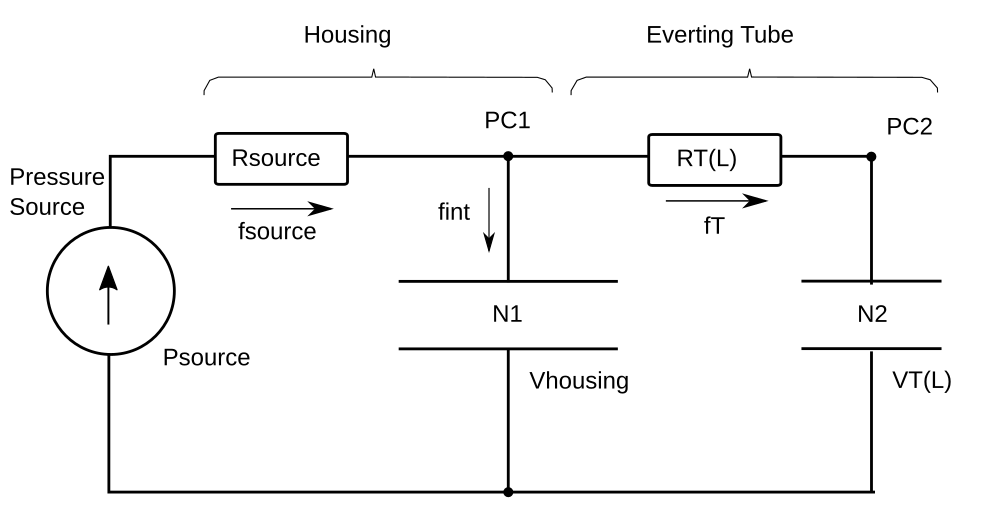
\includegraphics[width=.5\textwidth]{Figure_TwoCompartment.png}
\caption{Two compartment, lumped parameter model. }
\label{Fig:TwoCompartment}
\end{figure}

We need to expand our model state variables as follows:

\beq
\begin{aligned}
N, \dot{N}     &\to \{ N_1, N_2, \dot{N}_1, \dot{N}_2\}\\
V_{t}          &\to \{V_{housing}, V_T(L)\}\\
f_{source}     &\to \{f_{source}, f_{int}, f_{T} \}  \\
P              &\to \{ P_{C1}, P_{C2} \}
\end{aligned}
\eeq where
$N_1$ and $N_2$ are the molar quantity of air in the housing and tube respectively,
$f_i$ are the respective flows indicated in Figure \ref{Fig:TwoCompartment},
and
$P_{C1}$ and $P_{C2}$ are the pressures in the housing and tube respectivly.



We then have new equations to replace or expand Equations \ref{eqOneCompartmentPress}, \ref{eqOneCompartmentflow}, and \ref{eqOneCompartmentNdot}
as follows:

\beq
\dot{N_1} = f_{source}-f_{int}-f_T
\eeq

\beq
\dot{N_2} =  f_T
\eeq

\beq
P_{C1} = \frac {N_1RT}  {V_{housing}}
\eeq

\beq
P_{C2} = \frac {N_2RT}  {V_T(L)}
\eeq

\beq
f_{source} = (P_{source}-P_{C1}) /  R_{source}
\eeq

\beq
f_{T} = (P_{C1}-P_{C2}) /  R_{T}(L)
\eeq

\beq
f_{int} = f_{source} - f_T
\eeq

\section{Results of Two Compartment Model}

\begin{figure}[h]\centering
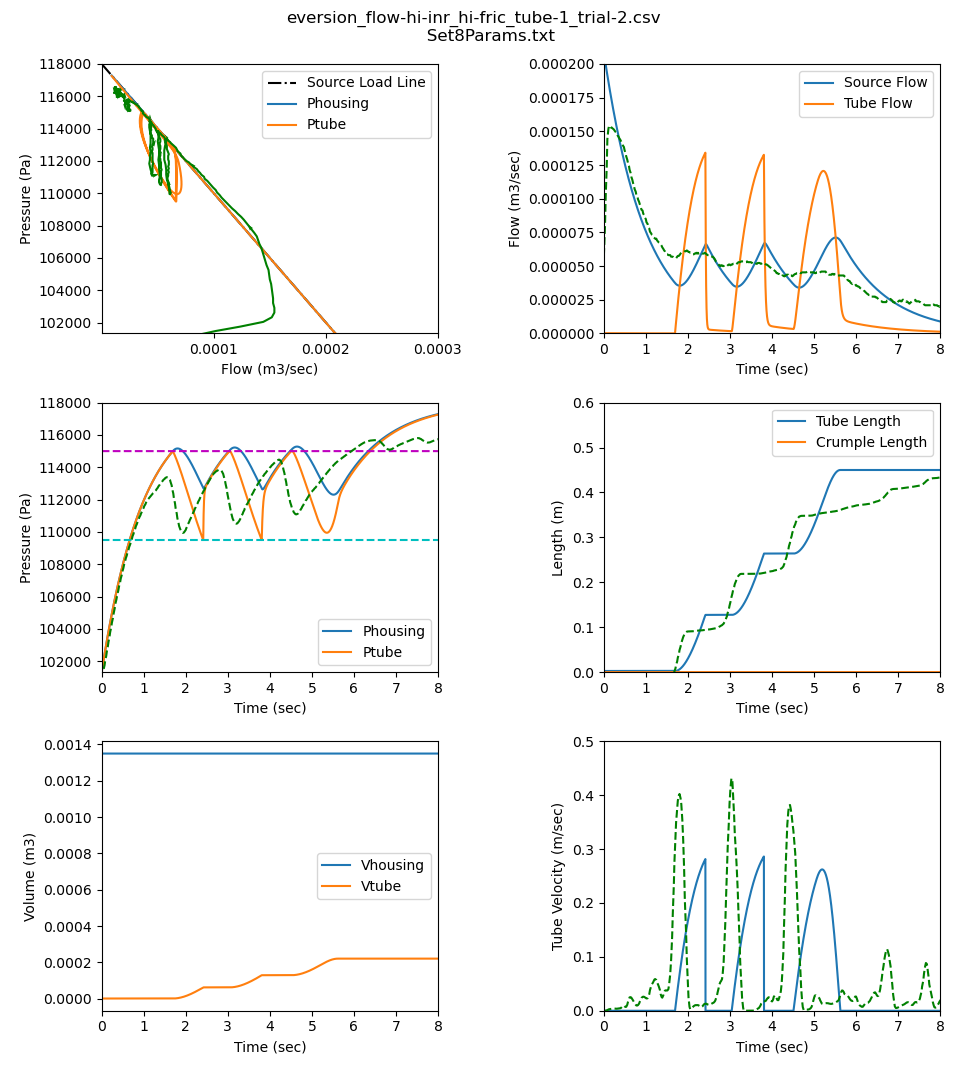
\includegraphics[width=.75\textwidth]{2CompSimulationSet8.png}
\caption{Two compartment model compared with simulation (See Lewis, Fig 9, hiI, hiTf)}
\label{Fig:2Comp}
\end{figure}


The data sets were simulated with the two-compartment version of the model.  Volume of the ET was
a function of length, $L$.  Flow resistance between reel housing (compartment 1) and
the ET was approximated by a ratio of Rsource\_SIu (typically 0.1).

Results from Tube 1, Trial 2 (hi inertia, hi friction) are given in Figure \ref{Fig:2Comp}.
Notably, the simulated tube pressure deviates below the source loadline during the start-stop
oscillations similar to the experimental data.
%  Use name of bibliography files without .bib extension
\bibliography{flowMOdel}
\end{document}
